\documentclass[10pt]{sigplanconf}
\usepackage{etex}

\usepackage{color}
\usepackage{balance}
\usepackage{amsmath}
\usepackage{stmaryrd}
\usepackage{graphicx}
\usepackage{amssymb}
\usepackage{fancyvrb}
\usepackage{url}
\usepackage{pstricks,pst-node,pst-tree}
\usepackage{theorem}
\usepackage{bbm}
\usepackage{pgf}
\usepackage{multirow}
\usepackage{rotating}
\usepackage{listings}
\usepackage{verbatim}
\usepackage{graphicx}
\usepackage{wrapfig}
\usepackage{xspace}
\usepackage{ql}
\usepackage{mdwlist}
\usepackage{morefloats}
\usepackage[T1]{fontenc}
\usepackage[scaled=0.85]{beramono}
\usepackage{dirtree}
\usepackage{booktabs}
\usepackage{mathptmx}
\usepackage[normalem]{ulem}
\usepackage[firstpage]{draftwatermark}
\SetWatermarkText{\hspace*{8in}\raisebox{3.9in}{
\includegraphics[scale=0.1]{aec-badge}}}
\SetWatermarkAngle{0}

\hyphenation{
Java Again since Gb fact parts ECOOP term
de-tails state-ments con-structs small-er ab-stract
im-ple-ment dif-fer-ent
im-ple-men-ta-tions gen-er-al-i-za-tions ex-pres-sions tra-vers-als Pro-gram-mers
}

\lstset{ %
language=Java,                % choose the language of the code
columns=flexible,
lineskip=-1pt,
basicstyle=\ttfamily\small,       % the size of the fonts that are used for the code
numbers=none,                   % where to put the line-numbers
numberstyle=\ttfamily\tiny,      % the size of the fonts that are used for the line-numbers
stepnumber=1,                   % the step between two line-numbers. If it's 1 each line will be numbered
numbersep=5pt,                  % how far the line-numbers are from the code
backgroundcolor=\color{white},  % choose the background color. You must add \usepackage{color}
showspaces=false,               % show spaces adding particular underscores
showstringspaces=false,         % underline spaces within strings
showtabs=false,                 % show tabs within strings adding particular underscores
%  frame=single,                   % adds a frame around the code
tabsize=2,                  % sets default tabsize to 2 spaces
captionpos=none,                   % sets the caption-position to bottom
breaklines=true,                % sets automatic line breaking
breakatwhitespace=false,        % sets if automatic breaks should only happen at whitespace
title=\lstname,                 % show the filename of files included with \lstinputlisting; also try caption instead of title
escapeinside={(*}{*)},          % if you want to add a comment within your code
keywordstyle=\ttfamily\bfseries,
deletekeywords={label}
% commentstyle=\color{Gray},
% stringstyle=\color{Green}
}

\pagestyle{plain}


\newcommand{\authornote}[3]{{\color{#2} {\sc #1}: #3}}
\newcommand\jason[1]{\authornote{jason}{green}{#1}}
\newcommand\haoyuan[1]{\authornote{haoyuan}{red}{#1}}
\newcommand\bruno[1]{\authornote{bruno}{red}{#1}}
\newcommand\tijs[1]{\authornote{tijs}{blue}{#1}}

\newcommand\name{{\bf Shy}\xspace}
\newcommand\Name{{\bf Shy}\xspace}

\newcommand{\hl}[1]{\textcolor{red}{#1}}

\newcommand\sem[1]{\llbracket #1 \rrbracket_r}
\newcommand\sems[1]{\llbracket #1 \rrbracket_s}
\newcommand\tsem[1]{\llbracket #1 \rrbracket}
\newcommand{\rbm}[1]{\raisebox{-2.0ex}[0.5ex]{#1}}
\newcommand\nat[0]{\mathbb{N}}
\newcommand\unit[0]{\mathbbm{1}}

\begin{comment}
\author{Author1$^{\textrm{1}}$ Author2$^{\textrm{2}}$ }
\institute{$^{\textrm{1}}$The University of Hong Kong\\
\email{author1@cs.hku.hk}\\
$^{\textrm{2}}$ The University of Hong Kong\\
\email{author2@cs.hku.hk}}
\authorrunning{Author1 and Author2} % abbreviated author list (for running head)
\end{comment}

\begin{document}
\toappear{}

\special{papersize=8.5in,11in}
\setlength{\pdfpageheight}{\paperheight}
\setlength{\pdfpagewidth}{\paperwidth}

\conferenceinfo{SPLASH '15}{October 25--30, 2015, Pittsburgh, Pennsylvania, USA.}
\copyrightyear{2015}
\copyrightdata{978-1-nnnn-nnnn-n/yy/mm}
\doi{nnnnnnn.nnnnnnn}

% Uncomment one of the following two, if you are not going for the
% traditional copyright transfer agreement.

%\exclusivelicense                % ACM gets exclusive license to publish,
                                  % you retain copyright

%\permissiontopublish             % ACM gets nonexclusive license to publish
                                  % (paid open-access papers,
                                  % short abstracts)

\titlebanner{banner above paper title}        % These are ignored unless
\preprintfooter{short description of paper}   % 'preprint' option specified.

\title{Scrap your Boilerplate with Object Algebras}
%\subtitle{Subtitle Text, if any}

\authorinfo{Haoyuan Zhang \and Zewei Chu \and Bruno~C.~d.~S.~Oliveira}
           {The University of Hong Kong}
           {\{hyzhang,jason91,bruno\}@cs.hku.hk}
\authorinfo{Tijs van der Storm}
           {Centrum Wiskunde \& Informatica (CWI)}
           {storm@cwi.nl}

\maketitle

\begin{abstract}

Traversing complex \emph{Abstract Syntax Trees} (ASTs) typically requires
large amounts of tedious boilerplate code. For many operations most of
the code simply walks the structure, and only a small portion of the
code implements the functionality that motivated the traversal in the
first place.  This paper presents a type-safe Java framework called
\name that removes much of this boilerplate code. In \name
\emph{Object Algebras} are used to describe complex and extensible
AST structures. Using Java annotations \name generates generic boilerplate code
for various types of traversals. For a concrete traversal, users of
\name can then inherit from the generated code
and override only the interesting cases. Consequently, the amount of code that users
need to write is significantly smaller. Moreover, traversals using the
\name framework are also much more \emph{structure shy}, becoming more
adaptive to future changes or extensions to the AST structure.
%An additional benefit of \name is that traversal code can be easily
%reused by extensions of the
To prove the effectiveness of the approach, we applied \name
in the implementation of a domain-specific questionnaire
language. Our results show that for a large number of traversals
there was a significant reduction in the amount of user-defined code.
%\bruno{Say something more about extensibility and type-safety!}

\begin{comment}

Static types are useful to distinguish between different kinds
of nodes in a structure and to prevent misuses. The
distinction between different types of nodes also means that code for
dealing with each type of node is needed. However, in large structures,
such as the Abstract Syntax Tree (AST) of a programming language,
the amount of required code can be a problem. For some operations,
which traverse large structures, most of the code amounts to recursively
delegating the traversal to the child nodes. Only for some nodes
of the structure the code needs to do something different. Still
the programmer needs to diligently and tediously write the error-prone
traversal code for all nodes.

In this paper we present a framework

This approach works well for many operations,
which need different (and non-trivial) code for each different type
of node

%Unfortunately, for some operations the interesting

%%In large structures,
%%such as the Abstract Syntax Tree (AST) of a programming language,
%%the code required to traverse the whole structure is proportionaly large.


The problem is particularly prominent
in statically typed languages, where the typing discipline
enforces strict distinctions between different cases

Operations that traverse complex structures often require large and
tedious amounts of boilerplate code. In those operations there are
typically a few

A pervasive problem in programming occurs when large tree tr

\end{comment}

\end{abstract}

\category{D.3.2}{Programming Languages}
                {Language Classifications}
                [Object-Oriented Programming]
\category{F.3.3}{Logics and Meanings of Programs}
                {Studies of Program Constructs}
                []

\terms
Languages

\keywords
Object algebras, boilerplate code, Java, adaptive object-oriented programming

%===============================================================================

\section{Introduction}

Various language processing tools or libraries for programming
languages, domain-specific languages, mark-up languages like HTML, or
data-interchange languages like XML or JSON require complex
\emph{Abstract Syntax Tree} (AST) structures. In those applications
ASTs are the key data structure needed to model the various constructs
of these languages. Such ASTs have various different types of nodes,
which can range from a few dozen to several hundred kinds of nodes
(for example in the ASTs of languages like Java or Cobol).

Static types are helpful to deal with such complex ASTs.  Static
types formalize the distinction between different kinds of
nodes. Furthermore the distinctions are helpful to ensure that
traversals over these ASTs have an appropriate piece of code
that deals with each different type of node. This can prevent a large
class of run-time errors that would not be detected otherwise.

%For example static types prevent errors that would arize from
%applying the code intended for a certain kind of node to another kind
%of node. Static types can also ensure that all nodes are dealt with by
%an appropriate piece of code.

Unfortunately, when traversing such ASTs, the number of nodes and the
enforced type distinctions between nodes can lead to so-called
\emph{boilerplate code}~\cite{ralf03syb}: code that is similar for most types of nodes and which
essentially just walks the structure. Operations where the ``interesting'' code is limited to only a small portion of nodes are called \emph{structure shy}~\cite{DemeterBook}.
A typical example is computing the free
variables of an expression in some programming language. In this
case, the interesting code occurs in the nodes representing the
binding and variable constructs. In all other cases, the code would just deal with
walking the structure. In ASTs with dozens or hundreds of
kinds of nodes, having to explicitly write code for each kind of node is both tedious and error-prone.
%In summary, structure shy operations
%suffer from the static typing discipline, because the type
%distinctions between different kinds of nodes leads to significant
%boilerplate code.

The boilerplate problem in implementing traversals has received
considerable attention in the past. For example, both \emph{Adaptive
  Object-Oriented Programming} (AOOP)~\cite{DemeterBook} and
\emph{Strategic Programming}~\cite{borovansky1996elan,visser1998core}
are aimed partly at solving this problem. Most approaches to AOOP and
strategic programming use some meta-programming techniques, such as
code generation or reflection. The use of meta-programming offers
programmers an easy way to avoid having to write boilerplate code.
This has important benefits: users have to write much less code; and
the code becomes much more adaptive to changes.
%Firstly the user has to write much less
%code, also removing the possibility of errors in the code walking the
%structure. Secondly the code becomes much more adaptive to changes: if
%a change to the traversed data type only affects the generated
%boilerplate code, the user-defined code can remain unchanged.
Nevertheless, such meta-programming based approaches usually come at the cost of
other desirable properties, such as type-safety, extensibility or
separate compilation. The functional programming community has also
studied the problem. For instance, the popular ``\emph{Scrap your
boilerplate}''~\cite{ralf03syb} approach supports type-safety and
separate compilation. Most of the techniques used in
functional languages, however, cannot be easily ported to mainstream OO
languages like Java, and are limited in terms of extensibility.


%Object
%algebras are a recently introduced technique, which has been shown to
%have significant advantages for software extensibility.

This paper presents a Java framework called \name that allows users to
define type-safe and extensible structure-shy operations. \name
uses \emph{Object Algebras}~\cite{bruno12oa} to describe ASTs, and to
write operations over ASTs in a style similar to writing folds in
functional programming. However unlike standard folds in
functional programming, Object Algebras are
\emph{extensible}: when new kinds of nodes are introduced in the data type, the operations can be extended as well, without changing existing code.

In \name Object Algebra interfaces are combined
with Java annotations to generate generic traversal code automatically. The
generated code accounts for four different types of traversals:
\emph{queries}; \emph{transformations}; \emph{generalized queries};
and \emph{contextual transformations}.  Each of these four types of
traversals is implemented as an Object Algebra. Programmers who want
to implement structure-shy traversals can then inherit from one of these
four Object Algebras, and override only the cases that deal with
the interesting parts of the traversal. 
Consequently traversals written in \name are:

\begin{itemize*}

\item {\bf Small in size:} With \name the amount of code that
  programmers need to write a structure-shy traversal is significantly smaller.
  Often traversals in \name are implementable in just a few lines
  of code, even for complex ASTs with hundreds of different types of
  nodes.

\item {\bf Adaptive and structure shy:}  Traversals written with \name can omit
  boilerplate code, making traversals more adaptive to
  future changes or extensions to the data type.

\item {\bf Type-safe:} \name traversals are directly written in Java
  and the Java type-system ensures type-safety. No run-time casts are
  needed for generic traversal code or for user-defined traversal
  code.

\item {\bf Extensible with separate compilation:} Traversals inherit type-safe
  extensibility from Object Algebras. Both traversals and the AST structures
  are extensible. Thus it is possible to
  reuse traversal code for ASTs extended with additional
  node types. Furthermore \name traversals support separate compilation.

\item {\bf Implemented in plain Java:} \name traversals do not require
  a new tool or language. The approach is library based and only uses
  Java annotations.

%\item {\bf Performant:} Traversals written with \name have performance that
%is comparable to naive hand-written OO code.

\end{itemize*}

\noindent To prove the effectiveness of the approach, we have applied \name in
the implementation of QL, a domain-specific language (DSL) for defining questionnaires that has been used before as a benchmark language~\cite{gouseti14extensible,erdweg2013state}.  Our results (see details in
Section~\ref{sec:case_study}) show that for a large number of traversals there was a
significant reduction in the amount of user-defined code: only 4\% to
21\% of the AST cases had to be implemented in comparison with code
written without \name.

Although \name's functional programming inspired idioms are new to
mainstream Java programmers, the use of standard Java constructs and techniques makes \name easy to implement, integrate in existing
environments, and use.  Moreover, although Java was chosen as the
implementation language for \Name, our approach should apply to any object-oriented
language with support for generics and annotations.

\begin{comment}

Existing work:

dynamic approaches: they can offer adaptivity and
structure shyness, but lack type-safety.

static approaches: No fully type-safe approach that we know
of for Java. Some approaches that rely on reflection and/or casts.
But these can have run-time type-errors and performance can be
quite bad.
Some static type-safe in the functional programming community,
but cannot be easily ported to Java (rely on sophisticated type
system features; target algebraic data types; ...). Moreover
(with a few exceptions) most approaches do not offer extensibility.

Static types are useful to distinguish between different kinds
of nodes in a structure and to prevent misuses. The
distinction between different types of nodes also means that code for
dealing with each type of node is needed. However, in large structures,
such as the Abstract Syntax Tree (AST) of a programming language,
the amount of required code can be a problem. For some operations,
which traverse large structures, most of the code amounts to recursively
delegating the traversal to the child nodes. Only for some nodes
of the structure the code needs to do something different. Still
the programmer needs to diligently and tediously write the error-prone
traversal code for all nodes.

In this paper we present a framework

This approach works well for many operations,
which need different (and non-trivial) code for each different type
of node

%Unfortunately, for some operations the interesting

%%In large structures,
%%such as the Abstract Syntax Tree (AST) of a programming language,
%%the code required to traverse the whole structure is proportionaly large.


The problem is particularly prominent
in statically typed languages, where the typing discipline
enforces strict distinctions between different cases

Operations that traverse complex structures often require large and
tedious amounts of boilerplate code. In those operations there are
typically a few

A pervasive problem in programming occurs when large tree tr

\end{comment}

In summary, the contributions of this paper are:

\begin{itemize*}

\item {\bf Design patterns for generic traversals.} We provide a set of design
patterns for various types of traversals using Object Algebras, including:
\emph{queries}, \emph{transformations},
\emph{generalized queries} and \emph{contextual transformations}.

\item {\bf The Shy Java framework.} We show that those design patterns
  can be automatically generated for a given Object Algebra
  interface. The \name framework\footnote{{\bf Available at:} \url{https://github.com/JasonCHU/SYBwithOA}} realizes this idea by using
   Java annotations to automatically generate generic traversals.

\item {\bf Applications and examples:} We show various 
  examples of traversals, such as free variables
  and substitution operations, implemented concisely with
  \name. Moreover we illustrate how certain
  kinds of \emph{desugarings} can be implemented using transformations, and
  how multiple transformations can be chained together in a \emph{pipeline}.

\item {\bf Case study.} We illustrate the benefits of \name using a case study based on the QL domain-specific
  language. The results of our case study show significant savings in
  terms of user-defined traversal code. The case study also shows that \name does not incur significant performance overhead compared to a regular AST-based implementation.
\end{itemize*}


\section{Object Algebras}\label{subsec:ObjectAlgebras}

Object Algebras capture a design pattern to solve the Expression Problem~\cite{wadler98expression-problem}.
As a result Object Algebras support modular and type-safe extensibility in two dimensions:
data variants and operations. Object Algebras can be used conveniently model recursive data types, such as ASTs. Here we briefly introduce Object Algebras using the example of a simple expression language. 

\begin{figure}[t]
\nocaptionrule
\lstinputlisting[linerange=4-7]{../ObjectAlgebras/src/example_object_algebras/ObjectAlgebras.java} % APPLY:linerange=INT_ALG_INTERFACE
\caption{A simple expression language}
\label{int_alg_interface}
\end{figure}

Fig.~\ref{int_alg_interface} shows an \emph{Object Algebra interface} which models \lstinline{lit} and \lstinline{add} expressions of \lstinline{ExpAlg}. The interface resembles abstract factory interface, but it instead of constructing objects of a concrete type, the result is abstract through the type parameter \lstinline{E}.
A concrete Object Algebra will implement such an interface instantiate the type parameter to construct objects for a particular purpose.

\begin{figure}[t]
\nocaptionrule
\lstinputlisting[linerange=27-34]{../ObjectAlgebras/src/example_object_algebras/ObjectAlgebras.java} % APPLY:linerange=EXP_FACTORY
\caption{Evaluating expressions}
\label{exp_factory}
\end{figure}

\begin{figure}[t]
\nocaptionrule
\lstinputlisting[linerange=38-45]{../ObjectAlgebras/src/example_object_algebras/ObjectAlgebras.java} % APPLY:linerange=INT_PRINT
\caption{Printing expressions}
\label{int_print_factory}
\end{figure}

For instance, Figure~\ref{exp_factory} shows a class implementing evaluation of expression.
Using this algebra to create expression in fact immediately evaluates the expression to its result.
To add another operation the interface is simply implemented again. As an example Figure~\ref{int_print_factory} shows the a simple printing operation on expressions.
Both examples illustrate extension in the dimension of operations.

%% \begin{figure}[t]
%% \nocaptionrule
%% \lstinputlisting[linerange=51-61]{../ObjectAlgebras/src/example_object_algebras/ObjectAlgebras.java} % APPLY:linerange=OA_TEST_CODE
%% \caption{Object Algebra Test Code}
%% \label{oa_test_code}
%% \end{figure}

\begin{figure}[t]
\nocaptionrule
\lstinputlisting[linerange=11-13]{../ObjectAlgebras/src/example_object_algebras/ObjectAlgebras.java} % APPLY:linerange=INT_BOOL_ALG_INTERFACE
\caption{Extending the language of expressions with multiplication}
\label{int_bool_alg_interface}
\end{figure}


\begin{figure}[t]
\nocaptionrule
\lstinputlisting[linerange=17-22]{../ObjectAlgebras/src/example_object_algebras/ObjectAlgebras.java} % APPLY:linerange=MUL_EVAL
\caption{Extending expression evaluation to support multiplication}
\label{mul_eval}
\end{figure}


The other dimension of extensibility (adding data variants) is  realized by extending the object algebra interface itself. Figure~\ref{int_bool_alg_interface} extends the original \lstinline{ExpAlg} with multiplication expressions.
The key feature of Object Algebras is that the existing operations (evaluation and printing) can now be extended to support multiplication without having to change the existing \lstinline{Eval} and \lstinline{Print} classes. Figure~\ref{mul_eval} shows how this is realized for evaluation. 

In summary, Object Algebra interfaces  describe recursive data types, and implementations of those interfaces represent operations. Extending the interface allows developers to extend the data type with new data variants, and (re)implementing the interface allows developers to define operations.
Finally, extension in both dimensions is fully type safe and does not compromise separate compilation.
%What makes \emph{object algebras} a useful design pattern even more is that it does not rely on any advanced language features, and it is both extensible and type-safe.


\begin{comment}

This paper showed how various types of traversals for complex
structures can be automatically provided by \Name. \name traversals are
written directly in Java and are type-safe, extensible and separately
compilable. There has always been a tension between the
correctness guarantees of static typing, and the flexibility of
untyped/dynamically-typed approaches. \name shows that even
in type systems like Java's, it is possible to get considerable
flexibility and adaptability for the problem of boilerplate code in
traversals of complex structures, without giving up modular static typing.
%\name offers the best of both worlds: the
%static typing guarantees; and flexibility and adaptability.

There are many of avenues for future work. One area of research is to
extend \name traversals to support flexible traversal strategies,
similarly to strategic
programming~\cite{borovansky1996elan,visser1998core,vandenBrand:2003:TRT:941566.941568}. Another
line of work worth exploring is to adopt generalizations of object
algebras~\cite{oliveira13fop} for added expressiveness of \name
traversals.

\end{comment}


\section{Overview}\label{subsec:overview}

This section starts by motivating the problem of boilerplate code in
traversals of complex structures. It then shows how \name addresses
the problem using a combination of object algebras~\cite{bruno12oa}
and Java annotations.

\subsection{A Questionnaire Structure and an Object Oriented Solution}

%Figure needed for the model.

%Duplicate texts.

We start by considering the questionnaire structure introduced in [Figure]. The example is actually closely based on our case study [Section], but appears in a much more simplified form to illustrate our work clearly. To start with, a questionnaire is rendered as an interactive form where, depending on user actions, new questions may appear, or values may be computed. A simplified DSL for questionnaires (QL), has its syntax in our example with a data structure. Three sorts of components, Form, Stmt and Exp help to compose questionnaires.

In the full QL structure, an identified \lstinline{Form} comprises a list of \lstinline{Statements}. Each \lstinline{Statement} can either be a question (a variable depending on users' input or assigned with an \lstinline{Expression}) or a condition statement. Furthermore, an \lstinline{Expression} is based on several primitive types, and is obtained from certain values, variables, together with some possible arithmetic operations. In this section, the simplified version of QL has only six constructors.

A concrete example QL questionnaire is shown in [Figure], regarding driver's license. The questionnaire firstly asks for a user's name and age, and for an adult, furthermore, it asks whether the user has a driver's license.

Two operations are supported by the QL structure: collecting the set of used variables in the questionnaire; and renaming all variables with an underscore ``\_'' appended to the end. To support those operations, an OO solution is to have methods \lstinline{usedVars}, which returns a set of strings representing used variables, and \lstinline{renaming}, which updates the names of all variables in a questionnaire.

[Figure] shows the Java implementation of this OO approach. In the implementation, collecting the set of used variables is done by returning the variable name in instances of the \lstinline{Var} class, and delegating the method \lstinline{usedVars} to the child nodes in other classes. Renaming variables asks the instances of the \lstinline{Question} and \lstinline{Var} classes to do the renaming task, and similarly, other classes just delegates the method \lstinline{renaming}. The renaming operation updates some information stored in the private members of those classes.

However, this simple OO solution has two important problems:

\begin{enumerate}

\item {\bf Lack of extensibility} The OO style
  representation of data structures is cumbersome and
  inflexible due to the bound relationship between classes. For
  instance, adding a new operation such as pretty
  printing the QL structure requires pervasive changes across all
  existing classes.

\item {\bf Boilerplate traversal code} Another issue is that we
  usually need to write a large amount of boilerplate code to
  implement traversals. In our example, we implemented
  \lstinline{usedVars} and \lstinline{renaming} in all
  classes. However only the \lstinline{Question} and \lstinline{Var} classes do some
  interesting work. All other classes simply delegate the task to the
  child nodes. This problem becomes more severe with bigger tree
  structures. The interesting code can become a very small portion of
  the code needed to perform a traversal: most of the code is doing
  tedious walking of the structure.

\end{enumerate}

\subsection{Modeling the QL Structure with Object Algebras}

Object algebras~\cite{bruno12oa} provide a solution to the extensibility problem.
Object algebras are a design pattern that is useful to model complex
structures, while providing a lot of flexibility in terms of
modularity and extensibility. In particular, object algebras allow
extensibility in two dimensions: it is easy to add new types of
nodes; and new operations over the structure.

[Figure] shows the approach to model the QL
structure as an object algebra interface. Each kind of node (\lstinline{Exp}, \lstinline{Stmt}, \lstinline{Form})
is represented as a type parameter. Each method in the object algebra interface models a
constructor of some node in the QL structure. For example the
method \lstinline{form} constructs an instance of a form; whereas the
method \lstinline{question} creates an instance of a statement. From an
object-oriented perspective the methods in the interface are factory
methods. For the reader familiar with functional programming, the
resemblance to constructors of  (a system of) algebraic data types should be clear.

Operations are defined by implementing the object algebra interface.
The following code show an implementation of the used variables
operation.

\begin{lstlisting}[numbers=none,mathescape=true]
class UsedVars implements QLAlg<Set<String>, Set<String>, Set<String>> {

	public Set<String> form(String id, List<Set<String>> statements) {
		Set<String> res = new HashSet<String>();
		for (Set<String> s : statements)
			res.addAll(s);
		return res;
	}

	public Set<String> iff(Set<String> cond, Set<String> then) {
		Set<String> res = new HashSet<String>(cond);
		res.addAll(then);
		return res;
	}

	public Set<String> question(String id, String label, String type) {
		return Collections.emptySet();
	}

	public Set<String> lit(int x) {
		return Collections.emptySet();
	}

	public Set<String> var(String varName) {
		return Collections.singleton(varName);
	}

	public Set<String> geq(Set<String> lhs, Set<String> rhs) {
		Set<String> res = new HashSet<String>(lhs);
		res.addAll(rhs);
		return res;
	}

}
\end{lstlisting}


The \lstinline{UsedVars} class provides an implementation for each
of the methods in the object algebra interface, which defines the
overall used variables operation. Since the result of collecting those
variables is \lstinline{Set<String>}, all the type parameters are set to
that type. Most of the method implementations simply traverse the
child nodes and accumulate the salaries. That is the case, for
example, for \lstinline{form}. The only method implementation that does
something different is \lstinline{var}, which returns the salary
argument.

For the renaming operation the result is itself a structure
with all variable names updated. The following code shows the
implementation:

\begin{lstlisting}[numbers=none]
class Renaming<E, S, F> implements QLAlg<E, S, F> {

	private QLAlg<E, S, F> alg;
	
	public Renaming(QLAlg<E, S, F> alg) { this.alg = alg; }
	
	public F form(String id, List<S> statements) {
		return alg.form(id, statements);
	}

	public S iff(E cond, S then) {
		return alg.iff(cond, then);
	}

	public S question(String id, String label, String type) {
		return alg.question(id + "_", label, type);
	}

	public E lit(int x) {
		return alg.lit(x);
	}

	public E var(String varName) {
		return alg.var(varName + "_");
	}

	public E geq(E lhs, E rhs) {
		return alg.geq(lhs, rhs);
	}

}
\end{lstlisting}

The class \lstinline{Renaming} is parameterized by three types,
which represent the kinds of nodes in the QL structure. Each
constructor needs to build an instance of the right type of nodes.
Note that, due to the lack of better type-inference in Java, there is
some repetition of type-annotations. In order to create the updated
QL structure another algebra called \lstinline{alg} is used.
Almost all the method implementations reconstruct the structure with
no changes using the methods in \lstinline{alg}. Two exceptions are the
methods \lstinline{question} and \lstinline{var}, where the structure is also reconstructed, but
the names are modified with ``\_'' appended to the end.

Although we solved the problem of extensibility with object
algebras, the traversal code is still lengthy and we are still writing
tedious traversal code. In those two operations, the only interesting code
is in the methods \lstinline{question} and \lstinline{var}. Ideally, we would like to write only
the code for the interesting cases, and somehow ``inherit'' the
remainder tedious traversal code.

\subsection{\Name: An Object Algebra Framework for Traversals}

To deal with the boilerplate problem we created \Name: a Java object
algebras framework, which provides a number of generic traversals at
the cost of a simple annotation. The key idea in \name is to
automatically create highly generic object algebras, which encapsulate
common types of traversals. In particular \name supports generic
\emph{queries} and \emph{transformations}. Those two types of
traversals are useful to capture, respectively, the used variables and
renaming operations.

With \Name, programmers just need to add the \lstinline{@Algebra} annotation
to the definition of \lstinline{QLAlg} to get the code for generic
queries and transformations. An example of that annotation is already
shown in [Figure]. With that annotation several classes
are generated automatically, including \lstinline{QLAlgQuery} and
\lstinline{QLAlgTrans}. Using those classes the code needed to write
the used variables and renaming object algebras is much
shorter. The code for the two operations is shown in
[Figure]. By implementing the
\lstinline{QLAlgQuery} and \lstinline{QLAlgTrans} classes, only the methods
\lstinline{question} and \lstinline{var} needs to be overridden: all the other methods,
which do a simple generic traversal, are inherited. For queries the
only extra thing a programmer has to do is to provide an instance of a
monoid, which is used to specify how to accumulate the results during
the traversal. Similarly, for transformations, the programmer needs to
pass an algebra for providing the constructors for the transformation
code.

Some client code is shown as follows: %, using those two algebras based on our framework.

\begin{lstlisting}[numbers=none]
<E, S, F> F makeQL(QLAlg<E, S, F> alg) {
	S s0 = alg.question("name", "What is your name?", "string");
	S s1 = alg.question("age", "What is your age?", "integer");
	E ifStmt = alg.geq(alg.var("age"), alg.lit(18));
	S thenStmt = alg.question("license", "Do you have a driver's license?", "boolean");
	S s2 = alg.iff(ifStmt, thenStmt);
	return alg.form("DriverLicense", Arrays.asList(s0, s1, s2));		
}
\end{lstlisting}

This method is used to create a particular QL structure, in the
usual object algebras style.
Using this QL structure, we can use the \lstinline{UsedVars}
and \lstinline{Renaming} to compute some information about the questionnaire:

\begin{lstlisting}[numbers=none]
UsedVars usedVars = new UsedVars();
	System.out.println(makeQL(usedVars));
	Renaming<Set<String>, Set<String>, Set<String>> renaming = new Renaming<Set<String>, Set<String>, Set<String>>(usedVars);
	System.out.println(makeQL(renaming));
\end{lstlisting}

The results give \lstinline{[age]} and \lstinline{[age_]}, which
is respectively the set of used variables before and after renaming.

The remainder of the paper provides the details and implementation
techniques used in \Name. Besides basic queries and transformations,
\name also supports two generalizations of these types of traversals
called \emph{generalized queries} and \emph{contextual transformations}.



\section{Queries}\label{sec:queries}

This section shows the ideas behind generic queries and how they are
implemented in \Name.  A query is an operation that traverses a
structure and computes some aggregate value. The inspiration for
queries comes from similar types of traversals used in functional
programming libraries, such as ``Scrap your
Boilerplate''~\cite{ralf03syb}.

%We motivate queries by walking through a number
%of different ways in which such operations are implemented.


The following code shows a variant of the type of expressions shown in
Section~\ref{subsec:ObjectAlgebras},
represented as the Object Algebra interface \lstinline{ExpAlg}.

\lstinputlisting[linerange=6-11]{../ObjectAlgebras/src/expDemo3/ExpAlg.java} % APPLY:linerange=EXP_ALG

\noindent We will use this
minimal Object Algebra interface throughout the rest of the paper to
illustrate the various different types of traversals supported by
\Name.  Three different kinds of nodes exist: a numeric literal, a
variable or the addition of two expressions. Queries are illustrated
by implementing an operation to compute the free variables in an expression.

\begin{comment}
As a specific type of Object Algebras, queries allow users to define
new operations handling a user-defined data structure\bruno{This
  definition of queries is just too broad. Please
look at papers like Syb to see how they describe queries and transformations}. A \textit{query
  algebra} is a class implementing an Object Algebra interface by a
top-down traversal throughout the hierarchy. It is something
supporting the program to gather information from the substructures of
a data type recursively, and make a response at the root node to the
query.
\end{comment}

\subsection{Boilerplate Queries}\label{subsec:freevars}

Figure~\ref{freevars_without_monoid} shows a
standard approach for computing free variables using Object Algebras\footnote{Here and in the following we will use interfaces with \lstinline{default}-methods (as introduced in Java 8) to combine queries and transformations using multiple inheritance.}.
A set of strings is used to collect the names of the free variables. The
\lstinline{Var} method returns a singleton set of \lstinline{s},
whereas the \lstinline{Lit} method returns an empty set. The
more interesting case is in the \lstinline{Add} method, where the two
sets are joined into one.

\begin{figure}[t]
\nocaptionrule
\lstinputlisting[linerange=9-21]{../ObjectAlgebras/src/expDemo2/FreeVars.java} % APPLY:linerange=FREEVARS_WITHOUT_MONOID
\caption{Free variables as an Object Algebra.}
\label{freevars_without_monoid}
\end{figure}
\begin{comment}
\bruno{put code in a figure, add a caption and refer
  to the figure in the text.}
\end{comment}

The typical pattern of a query is to collect some information from
some of the nodes of the structure, and to aggregate the information
that comes from multiple child nodes. For example, in the case of free
variables, the strings from the \lstinline{Var} nodes are collected,
and in the \lstinline{Add} nodes the information from multiple
children is merged into a single set.

An important observation about
queries is that the code to aggregate information tends to be the
same: if we had a subtraction node, the code would be essentially
identical to \lstinline{Add}. Moreover, there are only very few types
of nodes that contain relevant information for the query. For nodes
that contain information that is not relevant to the query, we simply
return \hl{\sout{the}} a neutral value (such as the empty set in \lstinline{Lit}).
Nonetheless, a programmer has to write this boring boilerplate code
handling the traversals.  While for the small structure presented here
this may not look too daunting, in a large structure with dozens or
even hundreds of constructors such code becomes a significant burden.

%Moreover, it is a query-based
%approach: you still have to write a bunch of similar stuff with a
%different query raised, for instance, a pretty printer.

\subsection{Generic Queries}\label{subsec:genericquery}

A better approach would be to abstract the generic traversal
and accumulation code for queries. This way, when programmers need to implement query
operations, they can simply reuse the generic traversal code and
focus only on dealing with the nodes that do something interesting.

%Queries are so similar actually: a user has to indicate the rules in
%which the program may address cases on primitive types and ``append''
%the information. With these two issues, everything becomes simple in
%the traversal. Hence we introduce the concept of monoid and generic
%traversal here in our query algebras.

%% \begin{figure}[tb]
%% \lstinputlisting[linerange=5-8]{../ObjectAlgebras/src/expDemo3/Monoid.java} % APPLY:linerange=MONOID
%% \vspace{-.1in}
%% \caption{The monoid interface.}
%% \label{monoid}
%% \end{figure}

The code that captures the aggregation and collection of information
can be captured by a well-known algebraic structure called a
\emph{monoid}. Monoids are commonly used in functional programming
for such purposes, but they are perhaps less commonly known in
object-oriented programming.  The interface of a monoid is defined as follows:
\begin{quote}
\lstinputlisting[linerange=5-8]{../ObjectAlgebras/src/expDemo3/Monoid.java} % APPLY:linerange=MONOID
\end{quote}
Intuitively, the \lstinline{join()} method is
used to combine the information from substructures, and
\lstinline{empty()} is an indicator of ``no information''.
%% The monoid interface also includes one additional operation
%% called \lstinline{fold}, which takes a list of \lstinline{R}
%% and returns an aggregated \lstinline{R}. Finally, note that
%% even though \lstinline{Monoid} is an interface, the
%% \lstinline{fold} operation is defined. This is a new feature
%% of Java 8 called default methods, which allow default implementations
%% of methods in interfaces.
Using the monoid operations alone, it is possible to write a generic
query. \hl{(Double quotes removed)} Figure~\ref{generic_query} shows how this is achieved. In
nodes that contain child nodes, such as \lstinline{Add}, the
information is aggregated using \lstinline{join}. In nodes that
contain other information, such as \lstinline{Var} and
\lstinline{Lit}, the query returns \lstinline{empty}.
This allows concrete queries to be implemented by overriding methods from multiple, different algebras.
%\hl{Note that the method \lstinline{m()} holding the monoid is named in lowercase, so that it won't clash with
%the uppercase constructors.}

\begin{figure}[tb]
\nocaptionrule
\lstinputlisting[linerange=4-11]{../ObjectAlgebras/src/expDemo3/ExpAlgQuery.java} % APPLY:linerange=GENERIC_QUERY
\caption{Generic queries using a monoid.}
\label{generic_query}
\end{figure}

\begin{comment}
And now we find everything goes in an easier way: we don't care about
what kind of query it is any more during the traversal. Despite
whether it asks for all the names of free variables or a printer
showing the hierarchy of an expression, at first we can simply
override the method \lstinline{m()}, which provides an instance of
\lstinline{Monoid}, in the return statement. As the next step, we only
need to override a few other methods to meet the requirements. This is
the progress, once we have such a template dealing with the traversal,
all query algebras can be addressed in a more concise way, which is
called the \textit{generic query algebra}.
\end{comment}

\subsection{Free Variables with Generic Queries}\label{subsec:solvingfreevars}

%% \begin{figure}[t]
%% \lstinputlisting[linerange=9-14]{../ObjectAlgebras/src/expDemo3/SetMonoid.java} % APPLY:linerange=FREEVARS_MONOID
%% \vspace{-.1in}
%% \caption{A monoid instance defined for sets.}
%% \label{freevars_monoid}
%% \end{figure}

The \lstinline{ExpAlgQuery} interface provides an alternative way to
define the free variables operation.  Since the result of free
variables is a set, the monoid returned by \lstinline{m()} is an
implementation of the \lstinline{Monoid} interface. For this case the following implementation \hl{\sout{would} suffices}:

\lstinputlisting[linerange=27-36]{../ObjectAlgebras/src/monoid/SetMonoid.java} % APPLY:linerange=SET_MONOID

\noindent The method
\lstinline{empty()} corresponds to the empty set, and
\lstinline{join()} is implemented as union.  Using this monoid the
free variables operation is defined as follows:

%As an alternative way to handle the freeVars query, the query algebra
%is going to be a sub-interface of \lstinline{ExpAlgQuery}, the generic
%algebra, with generic type to be \lstinline{List<String>}.

\lstinputlisting[linerange=7-15]{../ObjectAlgebras/src/expDemo3/FreeVars.java} % APPLY:linerange=FREEVARS_WITH_MONOID

\noindent There are two important differences to the implementation in
Figure~\ref{freevars_without_monoid}. The first difference is that the monoid to be used
needs to be specified. However, the code for the monoid is still
quite short (only requires two method implementations) and, more importantly,
it is highly reusable. Indeed the \lstinline{SetMonoid} is reused
throughout the paper on various examples of queries.
Because monoid instances are so general purpose, the \name library
already contains many common monoid implementations\hl{, so} users do not
usually have to
define these instances themselves.
The second difference is that now only the case for variables needs to
be defined: the other cases are inherited from
\lstinline{ExpAlgQuery}.

\begin{comment}
\haoyuan{Begin: client code.}
Now one can do some experiments with this approach. First comes an example of the expression built up like this:

\lstinputlisting[linerange=11-13]{../ObjectAlgebras/src/expDemo3/ExpTest.java} % APPLY:linerange=GEN_EXP

The method \lstinline{genExp()} just gives the expression \lstinline{x + (y + 2)}. And then an instance of \lstinline{FreeVars} is passed to \lstinline{genExp()} to get the names of free variables.
The result given by the following code is \lstinline{[x, y]}, which is a set of strings.

\lstinputlisting[linerange=19-20]{../ObjectAlgebras/src/expDemo3/ExpTest.java} % APPLY:linerange=CLIENTCODE_FREEVARS

\haoyuan{End: client code. x + (y + 2) and [x, y] in code style?}
\end{comment}

%% At this point it is interesting to analyze the benefits and drawbacks
%% of this approach. A clear benefit is that we have to define fewer cases
%% in specific queries. For large structures, this is can amount to
%% significantly less code. However we have to create the generic
%% classes for each Object Algebra interface as well as to use (and
%% perhaps define) some monoids. The monoid structures tend to be
%% quite general, so they can be reused accross multiple queries. For example
%% the set monoid is useful for any query that returns sets, not just
%% free variables. Therefore such monoids are typically included in
%% libraries, and do not need to be defined for each query.
%% For the code for the generic query itself (\lstinline{ExpAlgQuery})
%% it is nice that the code can be reused accross multiple
%% queries, but it still has to be defined. Furthermore the definition still
%% consists of boring and tedious code.

%Clearly if
%there are only a few types of nodes (as in our minimal example)
%and a few operations, the effort does not seem worthwhile. But

\begin{comment}
But the result for an expression can only be a null list based on the
monoid. Thus in the freeVars query, furthermore, we expect the
variables to store their names into a list, and by using the monoid,
freeVars can be implemented. See Figure~\ref{freevars_with_monoid}.


When the interface \lstinline{FreeVarsExpAlg} is used, an object of
the \lstinline{FreeVarsMonoid} is then created. As we can see, it is
needless for a user to write an exclusive traversal fully for a data
structure. Nothing but a monoid is required together with a few
methods being overwritten. And furthermore, a monoid can usually be
shared among query algebras with the same data type.
\end{comment}

%\subsection{Generic Queries in \name}

The traversal code in \lstinline{ExpAlgQuery} is entirely
mechanical and can be automatically generated.  This is precisely what
\name does. Annotating algebra interfaces, such as \lstinline{ExpAlg}, with the annotation \lstinline{@Algebra},
triggers automatic generation of generic query interfaces, such as \lstinline{ExpAlgQuery}.
%\name also provides implementatations of a number of common monoids over sets, lists, and numbers.
Figure~\ref{queryTemplate} shows the general template in \name for an algebra \lstinline[mathescape=true]{Alg<X$_1$, $...$, X$_n$>}, with constructors \lstinline[mathescape=true]{f$_1$, $...$, f$_m$}.
Note that interface \lstinline{Alg}$_Q$ extends \lstinline{Alg} so that all type parameters are unified as type \lstinline{R}.
All arguments to a constructor \lstinline[mathescape=true]{f$_j$} are combined with \lstinline{join} from the monoid \lstinline{m()}. Arguments with primitive types, like \lstinline{int}, \lstinline{boolean} or \lstinline{String}, are ignored by default.

\begin{figure}[ht]
\nocaptionrule
\begin{lstlisting}[mathescape=true]
interface Alg$_Q$<R> extends Alg<R,$...$,R> {
  Monoid<R> m();

  default R f$_j$(R p$_1$, $...$, R p$_k$) {
    return  m().join(p$_1$, m().join(p$_2$, $...$, m().join(
        p$_{k-1}$, p$_k$)$...$)));
  }
  $...$
}
\end{lstlisting}
\caption{Generic template for generic queries. \hl{(moved)}}
\label{queryTemplate}
\end{figure}



\section{Generalized Queries}\label{sec:generalizedQueries}

The previous section introduced simple queries where each constructor
contributes to a single monoid.  Recursive data types, however, often
have multiple syntactic categories, for instance expressions and
statements.  In such multi-sorted Object Algebras each sort is
represented by a different type parameter in the algebra interface.
In this section we present \textit{generalized queries}, where each
such type parameter can be instantiated to different monoids.
It turns out that, for some operations, this generalized version 
of queries is needed.

\begin{comment}
\haoyuan{General template. Some redundant texts.}
Figure~\ref{gQueryTemplate} shows the general template for \lstinline{Alg<X1, X2, ..., Xn>}.
Note that interface \lstinline{Alg}$_{GQ}$ extends \lstinline{Alg} and declares one monoid for each sort. As we cannot directly join a monoid over one type with a monoid over another type, for every constructor in \lstinline{Alg}$_{GQ}$, the arguments with different types from its return type are ignored.

\begin{figure}[t]
\begin{lstlisting}[mathescape=true]
interface Alg$_{GQ}$<X$_1$,$...$,X$_n$> extends Alg<X$_1$,$...$,X$_n$> {
  Monoid<X$_1$> m$_1$(); $...$; Monoid<X$_n$> m$_n$();

  default X$_i$ f$_j$(X$^1_p$ p$_1$, $...$, X$^k_p$ p$_k$) {
    X$_i$ res = m$_i$().empty();

    /* For all $s$ such that X$^s_p$ = X$_i$. */
    res = m$_i$().join(res, p$_s$);
    $...$
  }
  $...$
}
\end{lstlisting}
\caption{Generic template for generating boilerplate of generalized queries}
\label{gQueryTemplate}
\end{figure}
\end{comment}


\subsection{Example: data dependencies}
\label{subsec:depGraph}
%\subsection{Dealing with multiple sorts}

A simple example of a generalized query is the extraction of the data
dependencies between assignment statements and variables in simple
imperative programs.  To express this query, the simple
\lstinline{ExpAlg} is first extended with statements using the
\lstinline{StatAlg} interface of Fig.~\ref{statalg}.  The extension
consists of statement constructors for sequential composition
(\lstinline{Seq}) and assignment (\lstinline{Assign}).  The generated
default implementation of queries over statements is shown in
Fig.~\ref{LST:gstatquery}.  Note that the interface declares two
monoids,---one for each sort.  Since the \lstinline{Assign} and
\lstinline{Seq} constructors create statements, they return elements
of the \lstinline{mStat()} monoid.  Furthermore, because it is
impossible to automatically join a monoid over one type with a monoid
over another type, the \lstinline{e} argument in \lstinline{Assign}
is ignored.  As a result, a
concrete implementation has to override this case to deal with the
transition from expressions to statements.

\begin{figure}[t]
\lstinputlisting[linerange=7-10]{../ObjectAlgebras/src/trees/StatAlg.java} % APPLY:linerange=STATALG
\vspace{-.1in}
\caption{Statement Algebra Interface}
\label{statalg}
\end{figure}


\begin{figure}[t]
\lstinputlisting[linerange=7-11]{../ObjectAlgebras/src/deps2/G_StatAlgQuery.java} % APPLY:linerange=GSTAT_QUERY
\vspace{-.1in}
\caption{Default implementation of queries over many-sorted statement algebra}
\label{LST:gstatquery}
\end{figure}


%An example of a query over the multi-sorted statement algebra is the extraction of data dependencies from a program.

Data dependencies are created by assignment statements: for a
statement \lstinline{Assign(String x, Exp e)} method, the variable
\lstinline{x} will depend on all variables appearing in \lstinline{e}.
The result of extracting such dependencies can be represented as
binary relation (a set of pairs). In expressions we need to collect
the free variables, which can be stored in a set of strings.  Thus in
this traversal two monoids are involved: a monoid for a set of pairs
of strings; and a monoid for a set of strings.

To implement the extraction of data dependencies only two cases have to
be implemented: the variable (\lstinline{Var}) case from the
\lstinline{ExpAlg} signature; and the assignment (\lstinline{Assign})
case from the \lstinline{StatAlg} signature.  The implementation is
shown in Fig.\ref{deps2}.  Note that the \lstinline{Assign} case takes
the input \lstinline{Set<String> e} and uses it to create the
dependency relation.  The propagation of dependencies across
sequential composition is automatic, as is the propagation of the set
of variables through the different types of expressions.


\begin{figure}[t]
\lstinputlisting[linerange=12-17]{../ObjectAlgebras/src/deps2/DepGraph.java} % APPLY:linerange=DEPS2
\vspace{-.1in}
\caption{Dependency Graph with Generalized Query Algebra}
\label{deps2}
\end{figure}

\begin{comment}
\haoyuan{Begin: client code.}

\lstinputlisting[linerange=14-17]{../ObjectAlgebras/src/deps2/TestDepGraph.java} % APPLY:linerange=GEN_DEPGRAPH

\lstinputlisting[linerange=23-27]{../ObjectAlgebras/src/deps2/TestDepGraph.java} % APPLY:linerange=CLIENTCODE_DEPGRAPH

\haoyuan{End: client code.}
\end{comment}

%The difference between generalized queries and homogeneous queries is that each type parameter of an Object Algebra interface is possibly instantiated to a different monoid.
%If each parameter is instantiated to the same monoid, generalized queries are equivalent to the queries of the previous section, with one important difference: in the latter case, each sort is contributing to the same monoid.
%The default implementation thus can carry over, for instance, query results of expression into the result of statements.


\section{Transformations}\label{sec:transformations}
\label{retroimp}

Queries are a way to extract information from a data structure.
Transformations, on the other hand, allow data structures to be
changed. Just as with queries, we can distinguish code that deals with
traversing the data structure from code that actually changes the
structure. In this section we show how to avoid most traversal
boilerplate code in the context of transformations based on Object
Algebras.


\subsection{Boilerplate Transformations}\label{subsec:substvars}

A simple example of a transformation algebra, using the object
algebra interface \lstinline{ExpAlg}, is substituting expressions for
variables. A manual implementation based on Object Algebras is shown
in Fig.~\ref{substvars_without_id}.

\begin{figure}[t]
\nocaptionrule
\lstinputlisting[linerange=4-14]{../ObjectAlgebras/src/expDemo2/SubstVar.java} % APPLY:linerange=SUBSTVARS_WITHOUT_ID
\caption{A normal algebra-based implementation of variable substitution}
\label{substvars_without_id}
\end{figure}

The expression to be substituted, and the variable to substitute for
are computed by the methods \lstinline{e()} and \lstinline{x()}
respectively. \lstinline{expAlg()} is an instance of
\lstinline{ExpAlg} on which the transformation is based. Since Object
Algebras are factories, the transformation is executed immediately
during construction. For instance, calling \lstinline{Var("x")} on a
\lstinline{SubstVar} object with \lstinline{x()} returning
\lstinline{"x"} immediately returns the result of \lstinline{e()},
--- the original variable expression is never created. In the other
cases, the original structure is recreated in the algebra
\lstinline{expAlg()}.

Again we observe the problem of traversal-only boilerplate code: the
\lstinline{Lit} and \lstinline{Add} methods simply delegate to the
base algebra \lstinline{expAlg()} without performing any computation.

\subsection{Generic Traversal Code}

The boilerplate code in transformations can be avoided by creating a
super-interface containing default methods performing the traversal
(shown in Fig.~\ref{generic_transform}). A concrete transformation can
then selectively override the cases of interest. Variable substitution
can now be implemented as shown in Fig.~\ref{substvars_with_id}. In
this case, only the method \lstinline{Var()} is overridden.


\begin{figure}[t]
\nocaptionrule
\lstinputlisting[linerange=4-9]{../ObjectAlgebras/src/expDemo3/ExpAlgTransform.java} % APPLY:linerange=GENERIC_TRANSFORM
\caption{Traversal-only base interface for implementing transformations of expressions}
\label{generic_transform}
\end{figure}


\begin{figure}[t]
\nocaptionrule
\lstinputlisting[linerange=4-7]{../ObjectAlgebras/src/expDemo3/SubstVar.java} % APPLY:linerange=SUBSTVARS_WITH_ID
\caption{Implementation of variable substitution using \name}
\label{substvars_with_id}
\end{figure}


To execute substitution, the \lstinline{SubstVar} should be subclassed
(either anonymously or explicitly) with implementations for
\lstinline{x()}, \lstinline{e()}, and \lstinline{expAlg()}. The base
algebra \lstinline{expAlg()} could for instance be an algebra for
pretty printing the expression with the substitution applied. Note
that this allows pipelining of transformations: there is no reason
\lstinline{expAlg()} cannot return yet another transformation
algebra.

\begin{comment}
\haoyuan{Begin: client code.}

Here we also give the client code. With the same expression \lstinline{x + (y + 2)}, a \lstinline{SubstVar} object is created. The base algebra \lstinline{expAlg()} here is implemented with an instance of \lstinline{FreeVars}, and we also override \lstinline{x()} and \lstinline{e()} aiming to substitute another variable \lstinline{"z"} for \lstinline{"x"}. The code is as follows, where the result of execution becomes \lstinline{[y, z]}.

\lstinputlisting[linerange=28-33]{../ObjectAlgebras/src/expDemo3/ExpTest.java} % APPLY:linerange=CLIENTCODE_SUBSTVAR

\haoyuan{End: client code.}
\end{comment}


Just like in the case of queries, the traversal code in \lstinline{ExpAlgTransform}
is entirely mechanical and can be automatically generated by \Name.
Annotating algebra interfaces, such as \lstinline{ExpAlg}, with the
annotation \lstinline{@Algebra}, triggers automatic generation of
generic transformation interfaces. Fig.~\ref{trafoTemplate} shows
the general template for the generated code. Here
\lstinline{Alg}$_T$ extends \lstinline{Alg} with the same sorts. And
the base algebra \lstinline{alg()} is declared inside.

\begin{figure}[t]
\nocaptionrule
\begin{lstlisting}[mathescape=true]
interface Alg$_T$<X$_1$,$...$,X$_n$> extends Alg<X$_1$,$...$,X$_n$> {
  Alg<X$_1$, ..., X$_n$> alg();

  default X$_i$ f$_j$(X$^1_p$ p$_1$, $...$, X$^k_p$ p$_k$) {
    return alg().f$_j$(p$_1$, $...$, p$_k$);
  }
  $...$
}
\end{lstlisting}
\caption{Generic template for generating boilerplate of transformations}
\label{trafoTemplate}
\end{figure}


%Another important characteristic is that we can apply several transformations to the data structure before a query. This pattern is called the \textit{transformation pipeline}. Since the transformation algebra \lstinline{ExpAlgTransform<Exp>} is a sub-interface of \lstinline{ExpAlg<Exp>}, it creates any instance with the same type as the \lstinline{expAlg()} inside. Therefore a programmer can define a number of transformation algebras, and compose them in sequence, like a nested structure. At the meantime, a query algebra is passed to the innermost \lstinline{expAlg()}. In that case, the query is traversed recursively throughout the pipeline and eventually derives a certain composite transformation algebra.


%The \lstinline{SubstVarsExpAlg} is still generic, yet something like a pretty printer can be passed to the \lstinline{expAlg()} inside as a query, to display the results. Hence at this moment, a programmer doesn't need to write boilerplate code for traversals. The identity approach and the pipeline of transformations provide users with a generic transformation like a template.



\section{Contextual Transformations}\label{sec:contexttrans}

In the previous section, our identity approach introduces a simple template for transformations. When a transformation algebra is requested, users can just override some of the methods, to avoid building up the complete framework for traversals, which can be quite complicated with boring code. Moreover, we mention that transformation algebras show up with a transformation pipeline, and once a query is passed to the pipeline, all the information is visited, processed and integrated exactly along with the construction. However, some other transformations are special, in the sense that they work in a different way. They are called \textit{contextual transformations}. Literally, they need to deal with the context in a data structure.

We can see in the previous transformation algebras, namely ``non-contextual'' ones according to our classification, that those methods in an algebra are usually doing their own jobs, sharing no information and hence we handle them separately. But in other situations, we may need to interact with the context, and propagate some additional information everywhere accordingly.

\subsection{Capture-avoiding substitution: a contextual transformation}\label{subsec:captureavoidsubst}

A good example for the contextual transformation, is the \textit{capture-avoiding substitution} (SUBST, for convenience). \haoyuan{citation needed.} The SUBST is distinguished from our previous substitution algebra, in the sense that, for example, with an extension to the \lstinline{ExpAlg}, including lambda expressions and applications, the substitution should be able to avoid variable capture problems. As our object algebra interface is flexible with high extensibility, we create a new interface here as the extension to \lstinline{ExpAlg}. See Fig.~\ref{lam_alg}.

\begin{figure}[!htbp]
\lstinputlisting[linerange=4-7]{../ObjectAlgebras/src/example_LamAlg1/LamAlg.java} % APPLY:linerange=LAM_ALG
\vspace{-.1in}
\caption{Object algebra interface: \lstinline{LamAlg}}
\label{lam_alg}
\end{figure}

Now our expression algebra also supports lambdas and applications. So when we want to substitute a specified variable for a new expression, we shall be careful that those free variables should not be captured when replacement is applied. This is to preserve the equivalence in semantics during substitution.

An algorithm for SUBST is given by (\haoyuan{citation}). The idea is that, besides the variable and the substitutive expression, we should always maintain a set of free variables, as well as a mapping for renaming during a top-down traversal. Here we see the difference from some common transformations: we are passing additional information among substructures from top to the bottom, and update it sometimes according to the context inside.

We give a representative approach here as usual, which solves SUBST with respect to transformation algebras.

Firstly we define a custom interface named \lstinline{Subst} in Fig.~\ref{interface_subst}. It has only one method inside, which takes four arguments: the variable to be substituted as a \lstinline{String}, the resulting expression of type \lstinline{Exp}, the set of free variables, and the mapping for renaming.

\begin{figure}[!htbp]
\lstinputlisting[linerange=7-9]{../ObjectAlgebras/src/example_LamAlg1/Subst.java} % APPLY:linerange=INTERFACE_SUBST
\vspace{-.1in}
\caption{The interface \lstinline{Subst} with only one function inside}
\label{interface_subst}
\end{figure}

Then we have the interface \lstinline{Substitution} for SUBST. See Fig.~\ref{capture_avoid_without_id}. This interface inherits both \lstinline{ExpAlg} and \lstinline{LamAlg}, and at the same time implements all the methods from the two original interfaces. The first observation is that, since we are overriding those methods, the types and the number of arguments cannot be changed, even if we need more information to be propagated everywhere. So the idea comes that we can put the information inside the interface \lstinline{Subst}. As \lstinline{Subst} serves like a functional interface, when we consider the return type of the methods to be \lstinline{Subst}, we are actually passing functions. That is to say, functions play the role helping to pass ``information'' from one to another, and the information can be modified at any time when we apply the same method \lstinline{subst()} with input changed. As the second observation, let us seek the method \lstinline{Add()} for details. It returns an object of \lstinline{Subst} like an identity function, except that \lstinline{subst()} is applied to both \lstinline{e1} and \lstinline{e2} with arguments unchanged. It implies that the information is passed from the source to the two branches \lstinline{e1} and \lstinline{e2}. So it reflects the principle of a top-down traversal: the information is passed down from the source to all the substructures.
\haoyuan{The code in this section takes too much space, and disrupt the layout of diagrams temporarily. Should be put in something like Appendix?}

\begin{figure}[tb]
\lstinputlisting[linerange=7-43]{../ObjectAlgebras/src/example_LamAlg1/Substitution.java} % APPLY:linerange=CAPTURE_AVOID_WITHOUT_ID
\vspace{-.1in}
\caption{A normal algebra-based approach for SUBST}
\label{capture_avoid_without_id}
\end{figure}

\subsection{Generic traversal for contextual transformations}\label{subsec:genericcontexttrans}

Again, one may also come up with the same question: can we also generalize the procedure of traversals, just like the generic transformations that we discussed before? The answer is yes.

Fig.~\ref{context_trans_expalg} and Fig.~\ref{context_trans_lamalg} show the generic transformation code for \lstinline{ExpAlg} and \lstinline{LamAlg}, respectively. They are inspired from the identity approach as well. Both interfaces have two generic types A and B, where A specifies the type of the information we are to propagate, and B actually corresponds to \lstinline{expAlg()} and \lstinline{lamAlg()}. They are the algebras that a transformation follows with the identity approach. Therefore, here the generic type for \lstinline{ExpAlg} and \lstinline{LamAlg} is \lstinline{Function<A, B>}. For the contextual transformations that refer to a data structure with multiple generic types, we may have various return types and the \lstinline{Function} instance could be curried.

\begin{figure}[tb]
\lstinputlisting[linerange=6-17]{../ObjectAlgebras/src/example_LamAlg2/G_ExpAlgTransform.java} % APPLY:linerange=CONTEXT_TRANS_EXPALG
\vspace{-.1in}
\caption{Generic contextual transformation by hand for \lstinline{ExpAlg}}
\label{context_trans_expalg}
\end{figure}

\begin{figure}[tb]
\lstinputlisting[linerange=6-14]{../ObjectAlgebras/src/example_LamAlg2/G_LamAlgTransform.java} % APPLY:linerange=CONTEXT_TRANS_LAMALG
\vspace{-.1in}
\caption{Generic contextual transformation by hand for \lstinline{LamAlg}}
\label{context_trans_lamalg}
\end{figure}

As we can see, there are two identity transformation algebras for \lstinline{ExpAlg} and \lstinline{LamAlg}, respectively. And a user can simply override some of the methods instead of write a lot of boilerplates for traversals, which could be even worse with a complicated structure.

\subsection{Solving SUBST with generic transformation algebra}\label{subsec:solvingsubst}

With those templates for contextual transformations, we can now address SUBST in a different way. There is an issue here, if we implement the transformation algebra just using \lstinline{Function}, the type would be a curried \lstinline{Function} with depth four, since we need four variables to be propagated. Instead we again define a new interface here, called \lstinline{SubstArgs}. See Fig.~\ref{interface_substargs}.

\begin{figure}[tb]
\lstinputlisting[linerange=7-30]{../ObjectAlgebras/src/example_LamAlg2/SubstArgs.java} % APPLY:linerange=INTERFACE_SUBSTARGS
\vspace{-.1in}
\caption{The interface \lstinline{SubstArgs}}
\label{interface_substargs}
\end{figure}

With \lstinline{SubstArgs}, the code is further simplified. Fig.~\ref{capture_avoid_with_id} gives a solution to SUBST based on the generic transformation algebras above. We can see that only \lstinline{Lam()} and \lstinline{Var()} are overridden, while in other methods the information is simply passed down by default. And other methods are just auxiliary functions. Note that in some client code, to use this transformation interface, we may firstly pass algebras to \lstinline{expAlg()} and \lstinline{lamAlg()}, and then the transformation pipeline returns a variable of type \lstinline{Function<Subst<Exp>, Exp>}, where \lstinline{Exp} is a fixed type. As the final step, we apply it to an interface of \lstinline{Subst} to get the result.

\begin{figure}[tb]
\lstinputlisting[linerange=10-44]{../ObjectAlgebras/src/example_LamAlg2/Substitution.java} % APPLY:linerange=CAPTURE_AVOID_WITH_ID
\vspace{-.1in}
\caption{The contextual transformation for SUBST using generic algebras}
\label{capture_avoid_with_id}
\end{figure}


\section{Heterogeneous Transformations}\label{sec:heterotrans}

\hl{A new section.}

In Section~\ref{sec:transformations}, we presented transformations, as well as the generic traversals generated by \name. Although different constructors can be used in transforming a data structure, the generic transformations generated by \name are actually type-preserving. We can observe from a transformation algebra that the base algebra always has the same type as the structure to be transformed.

On the other hand, transformations between different types are also useful under some circumstances. For instance, the desugaring in developing a compiler usually involves two ASTs, and they are only similar in some constructors. In that case, transformations return a different type of the structure.

As an example, we still use the interface \lstinline{ExpAlg}. Consider a new constructor called \lstinline{Double}, which multiplies an expression by two. We present it as an Object Algebra interface:

\lstinputlisting[linerange=6-9]{../ObjectAlgebras/src/trees/DoubleAlg.java} % APPLY:linerange=DOUBLE_TREE

\noindent Note that one can also define \lstinline{DoubleAlg} with four constructors, including those three in \lstinline{ExpAlg}. But this implementation is more concise with \name framework.

An expression with type \lstinline{ExpAlg<Exp> & DoubleAlg<Exp>} can be created using four constructors, where a transformation can for example be desugaring the case \lstinline{Double(e)} into \lstinline{Add(e, e)}. The other cases just remain unchanged. Below is an implementation by hand:

\lstinputlisting[linerange=7-21]{../ObjectAlgebras/src/example_DoubleAlg1/Desugar.java} % APPLY:linerange=DESUGAR_DOUBLE

\noindent With the \name framework one can easily implement \lstinline{Desugar} as follows: \hl{(add generated code to Appendix?)}

\lstinputlisting[linerange=7-12]{../ObjectAlgebras/src/example_DoubleAlg2/Desugar.java} % APPLY:linerange=DESUGAR_DOUBLE_SHY

\noindent Now one can create a structure of an expression with desugaring applied as follows:

\lstinputlisting[linerange=9-15]{../ObjectAlgebras/src/example_DoubleAlg2/Test.java} % APPLY:linerange=MAKE_DOUBLE_EXP

\noindent Here an expression ``\lstinline{5 + 2a}'' is created before transformation is applied. The base algebra \lstinline{alg} can for example be a pretty printer. By invoking this \lstinline{makeExp} method, a pretty printer can now return the result \lstinline{(5 + (a + a))}.




\section{Extensible Queries and Transformations}
\label{SECT:extensible}


\noindent \name queries and transformation inherit  modular extensibility from the Object Algebra design pattern.
New transformations or queries are simply added by extending the interfaces generated by \name.
More interestingly, however, it is also possible to extend the data type with new constructors.
Here we briefly describe how queries and transformations can be extended in this case.


Consider again the extension of the expression language with a lambda and application constructs (cf. Section~\ref{sec:contexttrans}).
This requires changing the free variables query, since variables bound by \lstinline{Lam} expressions need to be subtracted from the set of free variables of the body.
Instead of reimplementing the query from scratch, it is possible to modularly extend the existing \lstinline{FreeVars} query:

\lstinputlisting[linerange=18-22]{../ObjectAlgebras/src/expDemo3/FreeVarsWithLambda.java} % APPLY:linerange=EXTENDFREEVARS

The interface \lstinline{FreeVarsWithLambda} extends both the original \lstinline{FreeVars} query and the base query implementation that was generated for the \lstinline{LamAlg} interface defining the language extension.
Note again, that only the relevant method (\lstinline{Lam}) needs to be overridden. 


For transformations the pattern is similar.
To illustrate extension of transformation, consider the simple transformation that makes all variable occurrences unique.
This can be useful to distinguish multiple occurrences of the same name.

%% weird, computepositions does not compute the right range.
\lstinputlisting[linerange=4-2]{../ObjectAlgebras/src/expDemo3/Unique.java} % APPLY:linerange=UNIQUEVARS

The \lstinline{Unique} transformation uses a helper method \lstinline{nextInt()} which returns consecutive integers on each call.
The basic transformation simply renames \lstinline{Var} expressions.
If, again, the expression language is extended with lambda constructs, the transformation needs to be updated as well to make the variable in the binding position of lambda expression unique.
The following code shows how this can be done in a modular fashion:

\lstinputlisting[linerange=4-6]{../ObjectAlgebras/src/expDemo3/UniqueWithLambda.java} % APPLY:linerange=EXTEND_UNIQUEVARS

\noindent Note that the transformation uses the \lstinline{lamAlg()} algebra (from \lstinline{LamAlgTransform}),
to create lambda expressions.


\begin{figure}[t]
  \centering

  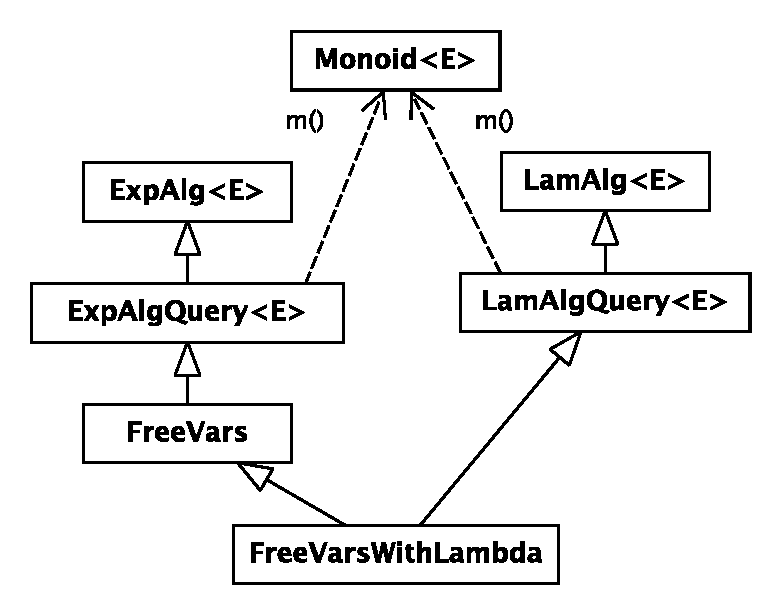
\includegraphics[width=0.45\linewidth]{extendQuery}
  \hspace*{2pt}
  \vline
  \hspace*{2pt}
  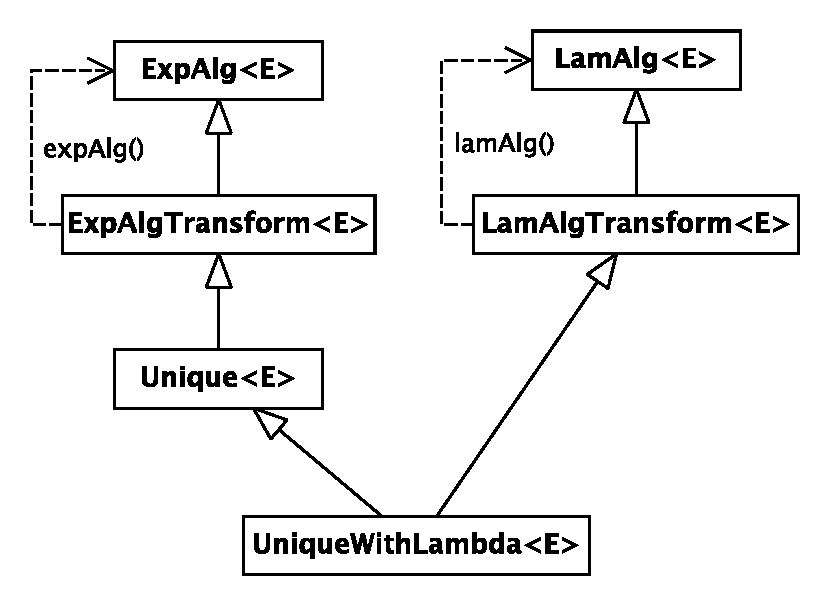
\includegraphics[width=0.45\linewidth]{extendTransform}
  
  \caption{Extension of the \lstinline{FreeVars} query (left) and the \lstinline{Unique} transformation (right)}
  \label{FIG:extension}
\end{figure}


Figure~\ref{FIG:extension} gives a high level overview of query and transformation extension using the examples for \lstinline{FreeVars} and \lstinline{Unique}. 
In the case of queries, the abstract \lstinline{m()} method will be shared by both the \lstinline{FreeVars} and \lstinline{FreeVarsWithLambda} interfaces.
On the other hand, transformations are based on multiple base algebras, for sets of data type constructors (e.g., \lstinline{expAlg()} and \lstinline{lamAlg()}). 

Note finally that, in the current implementation of \name transformations, it is assumed that the language signatures \lstinline{ExpAlg} and \lstinline{LamAlg} are completely independent.
This is however, not an essential requirement.
An alternative design could have \lstinline{LamAlg} be a proper extension of \lstinline{ExpAlg} (i.e. \lstinline{LamAlg<E> extends ExpAlg<E>}).
In that case, the generated \lstinline{LamAlgTransform} would need to refine the return type of the \lstinline{expAlg()} method. 




\section{Object Algebras Framework}

Generic queries and transformations can help users write tree structure traversal code with more extensibility and flexibility. However, writing the generic query and transformation interfaces is still painful experience by itself. It will be even better if these boilerplate code can be generated automatically. If we pay more attention to our generic query and transformation interfaces, without much difficulty we can find that the query and transform code structures for all \emph{Object Algebra Interfaces} are quite similar. Therefore we can make this code generation process automatic. 

To address this problem, we provide an \emph{Object Algebra Framework}, which utilizes \emph{Java Annotation} to generate generic query and transformation interfaces based on the \emph{Object Algebra Interface}. as illustrated below: 
\begin{lstlisting}[numbers=none] 
@Algebra
public interface ExpAlg<Exp> {
	Exp Var(String s);
	Exp Lit(int i);
	Exp Add(Exp e1, Exp e2);
}
\end{lstlisting}

With the annotation "$@$Algebra", the framework will generate the boilerplate codes for us automatically. As for our ExpAlg example, the following directory structure will be generated by the library. 
\dirtree{%
 .1 src/.
 .2 query/.
 .3 ExpAlgQuery.
 .2 transform/.
 .3 ExpAlgTransform.
}

Here the automatically generated ExpAlgQuery, ExpAlgTransform are exactly the same code as we discussed in Section~\ref{sec:queries} and Section~\ref{sec:transformations}. Furthermore, the monoid interface is also included in the \emph{Object Algebra Framework}.

Hence when programming with query, the programmer can skip the intermediate steps such as constructing generic queries and transformations, but only focus on rewriting the interesting cases. For instance, in our ExpAlg example, to implement FreeVars algebra, we can simply override the Exp Var(String s) method of ExpAlgQuery class to return variable name, and provide the specific monoid needed, which in this case will be a String List monoid. While the SubstVars algebra can be realized by overriding the Exp Var(String s) method of ExpAlgTransform interface, which substitutes variable names as specified. 


\section{Case Study}

We have used the Object Algebras framework in the implementation of a simple DSL for Questionnaires, called QL~\cite{gouseti14extensible}.
A questionnaire is rendered as an interactive form where, depending on user actions, new questions may appear, or values may be computed.
An example QL questionnaire is shown on the left of Fig.~\ref{FIG:houseowning} together with its rendering on the right.

QL programs consist of lists of labeled, typed questions.
Questions can be answerable, meaning the user has to enter some data, or computed.
In the latter case the question is defined by an expression.
A conditional if-then-else construct allows questions to visually appear only when a certain condition is true.

\begin{figure}[t]
\hspace*{-5pt}\begin{minipage}{0.6\linewidth}
\begin{lstlisting}[language=ql]
form HouseOwning {
  soldHouse: "Did you sell a house?" boolean
  boughtHouse: "Did you buy a house?" boolean
  if (soldHouse) {
    sellingPrice: "Selling price:" integer
    privateDebt: "Private debts:" integer
    valueResidue: "Value residue:" integer 
       = (sellingPrice - privateDebt)
  }
}
\end{lstlisting}
\end{minipage}
\begin{minipage}{0.5\linewidth}
  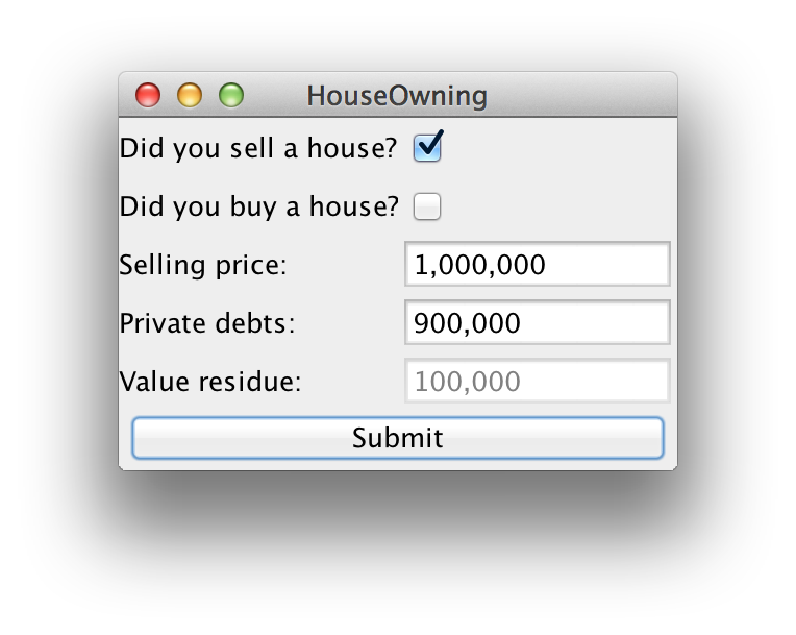
\includegraphics[width=\linewidth]{sections/screenshot}
\end{minipage}
\caption{Example QL questionnaire (left) and its rendering (right)}
\label{FIG:houseowning}
\end{figure}


To illustrate the utility of \name we have implemented a number of queries and transformations in the context of QL. The queries extract derived information from a QL program, such as the set of used variables, the data and control dependencies between questions and the type environment.
The transformations include two transformations of language extensions to the base language.
The first realizes a simple desugaring of ``unless(c){...}'' to ``if(not(c)){...}''.
The second desugaring statically unfolds a constant bound loop construct (``repeat (i){...}'') and renames variables accordingly.
Finally, we have implemented a simple rename variable operation, and a normalizer which inlines the conditions of nested if-then constructs.  

Table~\ref{TBL:qlresults} shows the number of cases that had to be overridden to implement each particular operation. The top row shows the number of  constructs for each sort in QL (Exp, Stmt, and Form, respectively).
As can be seen, none of the operations required implementing all cases.
For this set of queries and transformations, almost no expression cases needed to be overridden, except the ``Var'' case in collect variables, rename variable and desugar ``repeat''\footnote{Note, however, that the dependency extraction queries reuse the collect variables query on expressions.}.
The cases required for desugaring include the case of the language extension, which is not counted in the total in the top row. 

\begin{table}[t]
  \centering
  \begin{tabular}{l|c|c|c}
    Operation            & Exp (18) & Stmt (5) & Form (1) \\\hline
    Collect variables    & 1              &                &               \\
    Data dependencies    &                & 3               & 1             \\
    Control dependencies &                & 4              & 1             \\
    Type environment     &                & 2              &               \\\hline
    Rename variable      & 1              & 2              &               \\
    Inline conditions    &                & 4              &               \\
    Desugar ``unless''   &                & 1              &               \\
    Desugar ``repeat''   & 1              & 3              &               \\
  \end{tabular}
  \caption{Number of overriden cases per query and transformation in
    the context of the QL implementation\label{TBL:qlresults}}
\end{table}


\subsection{Extending queries and transformations}

Instead of desugaring language extensions to the base language it is also possible to treat them as first-class constructs and retroactively extend existing queries and transformations.
The framework permits to use  Java interface extension to achieve this in a fully type safe way.
Figure~\ref{inline_conds_unless} and Fig.~\ref{controldeps_unless} show the extension of the inline conditions transformation and control dependencies query when extending QL with ``unless''.

\begin{figure}[tb]
\lstinputlisting[linerange=9-14]{../QL/src/_syb/trafo/InlineConditionsUnless.java} % APPLY:linerange=INLINECONDS_UNLESS
\vspace{-.1in}
\caption{Extending the inline-conditions transformation to deal with ``unless''}
\label{inline_conds_unless}
\end{figure}

\begin{figure}[tb]
\lstinputlisting[linerange=10-18]{../QL/src/_syb/query/ControlDepGraphUnless.java} % APPLY:linerange=CONTROLDEPS_UNLESS
\vspace{-.1in}
\caption{Extending the control-dependencies query to deal with ``unless''}
\label{controldeps_unless}
\end{figure}

Inlining of conditions across ``unless'' statements (Fig.~\ref{inline_conds_unless}) is analogous to the implementation for ``if''.
It involves creating a conjunction of the input (\lstinline{guard}) and the negated condition and then passing it down the body of ``unless''. The result is the inlined version of the body.
The extension of the control dependencies (Fig.~\ref{controldeps_unless}) query simply delegates to the implementation of ``if'' (\lstinline{iff}). 

\subsection{Chaining transformations}

Transformations can be chained by passing transformation algebras as the base algebra to the implementation of another transformation.
For instance, the desugar unless transformation desugars the ``unless'' statement to ``if'' statements in another algebra.
Assuming this transformation is implemented by \lstinline{Desugar},  \lstinline{Inline} represents the inline conditions transformation, and \lstinline{Rename} represents the rename variable transformation. All three can be chained as follows:

  \lstinputlisting[linerange=162-162]{../QL/src/_syb/trafo/TestPipelining.java} % APPLY:linerange=PIPELINEQL

The chained transformation \lstinline{alg} first desugars ``unless'', then inlines conditions, and finally renames variables according to the map \lstinline{ren}.
The \lstinline{Rename} transformation gets as base algebra an instance of \lstinline{Format}, a pretty printer for QL. 

The algebra \lstinline{alg} can now be used to create questionnaires:

  \lstinputlisting[linerange=166-168]{../QL/src/_syb/trafo/TestPipelining.java} % APPLY:linerange=PIPELINEQL_CALL

The result of constructing this simple questionnaire is a function object representing the ``to be inlined'' representation of the questionnaire desugaring.
The \lstinline{IFormatWithPrecedence} and \lstinline{IFormat} types are  formatting operations, respectively representing expressions and statements; these types originate from the \lstinline{Format} algebra passed to \lstinline{Rename}.
Calling this function with a boolean expression representing \lstinline{true} will trigger inlining of conditions. The result is then a formatting object (\lstinline{IFormat}) which can be used to print out the transformed questionnaire:

  \begin{lstlisting}[language=ql]
    form myForm {
      if (true && !y) y "X?" boolean
    }
  \end{lstlisting}

As can be seen, the condition \lstinline{y} is now negated, because of the desugaring of ``unless''.
The result of inlining conditions can be observed from the conjunction in the \lstinline[language=ql]{if} statement. Finally, the variable \lstinline{x} has been renamed to \lstinline{y}.
  
\subsection{\name performance vs Vanilla ASTs}

\begin{figure}[t]
  \hspace*{-.1\textwidth}
  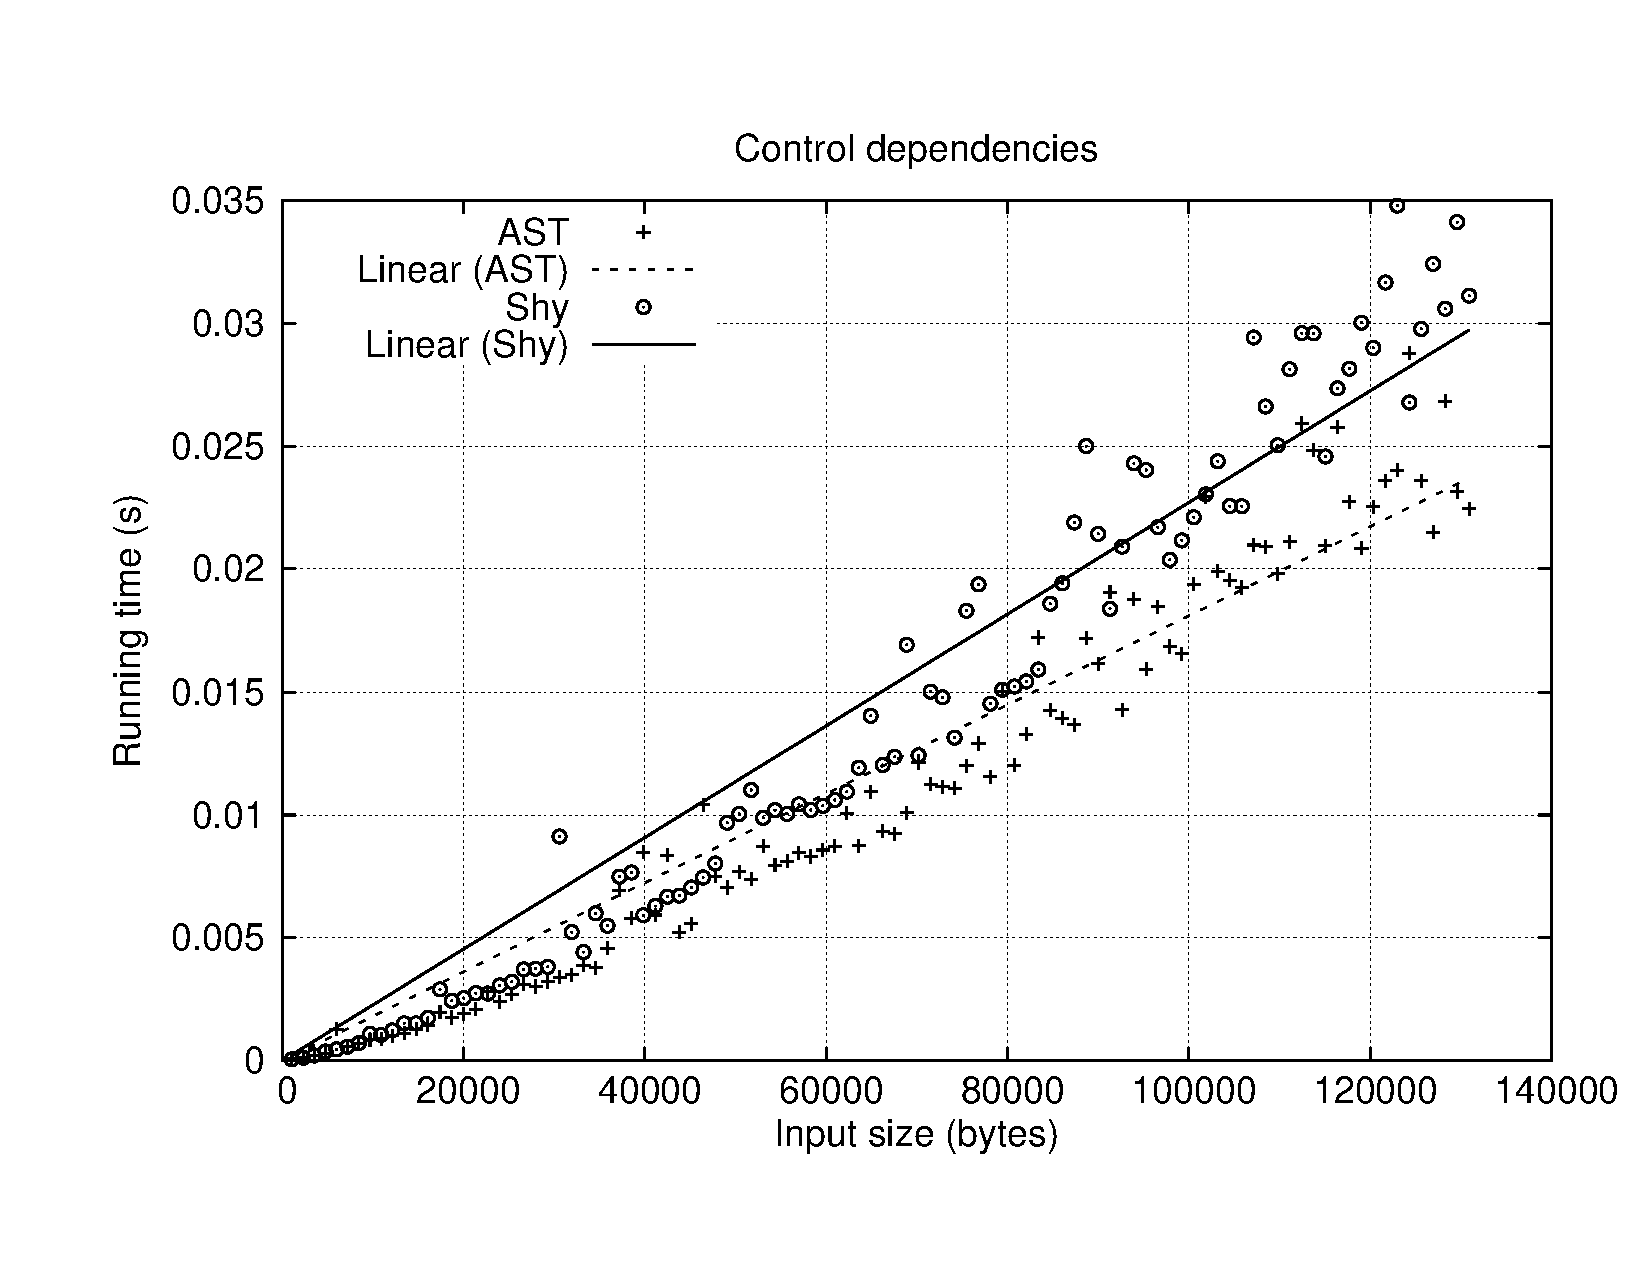
\includegraphics[width=0.56\textwidth]{plots/controldeps}
  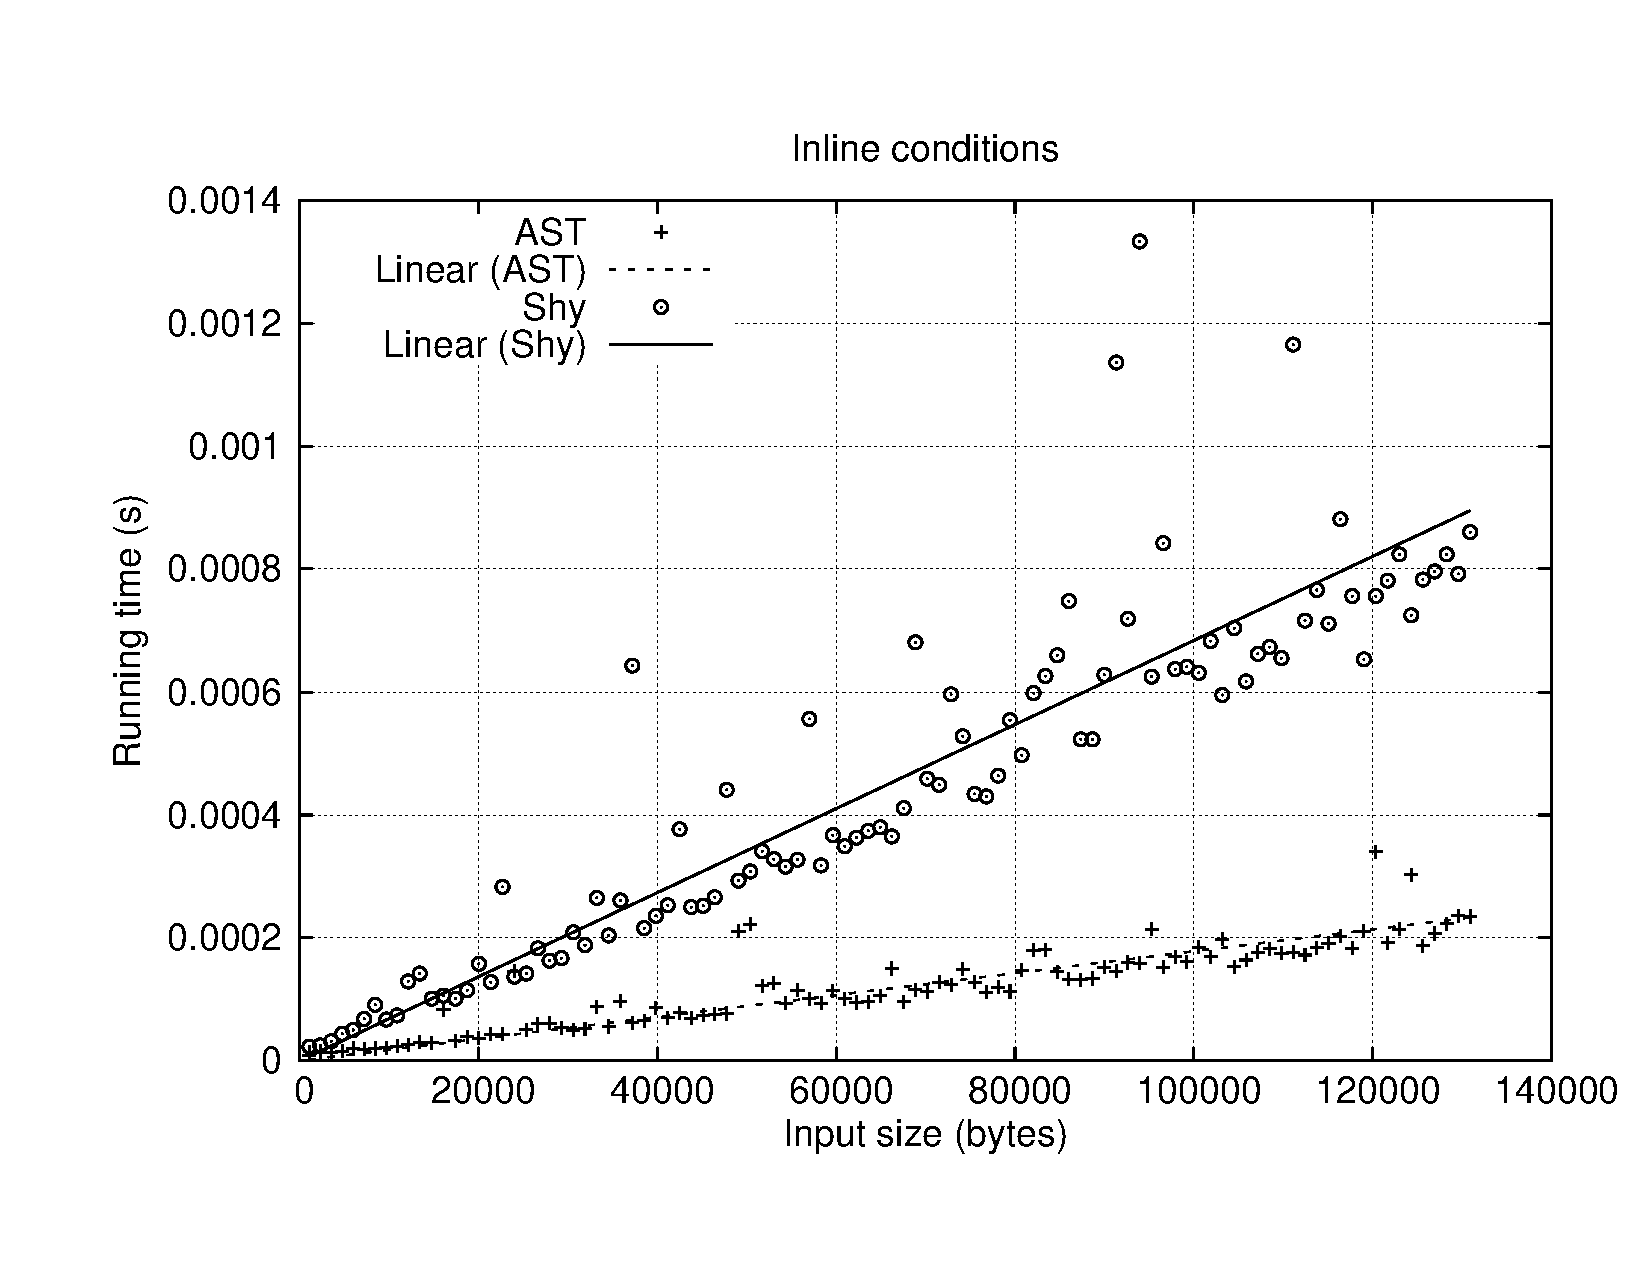
\includegraphics[width=0.56\textwidth]{plots/inline}
  \caption{Performance comparison of control dependencies query (left) and inline conditions transformation (right) implemented using normal ASTs vs using the \name framework\label{FIG:performance}}
\end{figure}

We compared the performance characteristics of the operations implemented using \name with respect to vanilla implementations based on ordinary AST classes.
The operations were executed on progressively larger QL programs (up to 140Kb).
In the vanilla implementation, the program was parsed into an AST structure, and then the operation was invoked and measured.
In the case of the \name queries, constructing the ``AST'' corresponds to executing the query, so we measured that.
For context-dependent transformation, however, building the ``AST'' corresponds to constructing the function to execute the transformation, hence we only measured the execution of invoking this function. 
To make the comparison as fair as possible, the query implementations use the same monoid structures as in \name.

The comparison of the control dependencies query is shown on the left of Fig.~\ref{FIG:performance}.
The plot shows that the performance is quite comparable.
On average, the \name implementation of the query seems a little slower.
This is probably caused by the extensive use of interfaces in the \name framework, whereas the AST-based implementation only uses abstract and concrete classes
%\tijs{NEED REFERENCE!!!!, but see: \url{http://stackoverflow.com/questions/6839943/why-are-interface-method-invocations-slower-than-concrete-invocations}}.

For transformations the performance difference is slightly more pronounced.
The right of Fig.~\ref{FIG:performance} shows the performance comparison of the inline conditions transformation. 
The greater difference can be explained by the fact that creating a new structure in a \name transformation involves dynamically dispatched method calls instead of statically bound constructor calls. 






\section{Related Work}\label{sec:related}

Finally related work.

\section{Conclusion}\label{sec:conclusion}

This paper showed how various types of traversals for complex
structures can be automatically provided by \Name. \name traversals are
written directly in Java and are type-safe, extensible and separately
compilable. There has always been a tension between the
correctness guarantees of static typing, and the flexibility of
untyped/dynamically-typed approaches. \name shows that even
in type systems like Java's, it is possible to get considerable
flexibility and adaptability for the problem of boilerplate code in
traversals of complex structures, without giving up modular static typing.
%\name offers the best of both worlds: the
%static typing guarantees; and flexibility and adaptability.

There are many avenues for future work. One area of research is to
extend \name traversals to support flexible traversal strategies,
similarly to strategic
programming~\cite{borovansky1996elan,visser1998core,vandenBrand:2003:TRT:941566.941568}. Another
line of work worth exploring is to adopt generalizations of object
algebras~\cite{oliveira13fop} for added expressiveness of \name
traversals.



\acks

We would like to thank T. H. Tse for valuable feedback on previous
drafts of this work. This work has been sponsored by the
Hong Kong Research Grant Council Early Career Scheme
project number 27200514 (``ALGEBRA: A Programming Language for Developing Software
Product Lines based on Object Algebras'').

\bibliographystyle{abbrvnat}
\bibliography{paper}


\appendix
\clearpage

\section{Appendix}\label{sec:appendix}

\subsection{Complete Code}

\subsubsection{OO Approach for \lstinline{usedVars} and \lstinline{rename}}\label{subsec:appendix_code_oo_approach}

Below is the complete code for Fig.~\ref{LST:usedVars} (left). It implements \lstinline{usedVars} and \lstinline{rename} in the QL example, as an OO approach.

\lstinputlisting[linerange=12-119]{../ObjectAlgebras/src/example_QLAlg1/QL.java} % APPLY:linerange=OO_APPROACH

\subsubsection{\lstinline{Rename} implementing the \lstinline{QLAlg} interface}\label{subsec:appendix_code_rename}

The following code gives the implementation of \lstinline{Rename} that implements \lstinline{QLAlg} in Section~\ref{subsec:model_ql_with_oa}.

\lstinputlisting[linerange=8-33]{../ObjectAlgebras/src/example_QLAlg2/Rename.java} % APPLY:linerange=QL_TRANSFORM_ALG

\begin{comment}
\subsubsection{\lstinline{SetMonoid}}\label{subsec:appendix_code_setmonoid}

The implementation of \lstinline{SetMonoid} for Fig.~\ref{ql_with_oaframework} and Section~\ref{subsec:solvingfreevars}.

\lstinputlisting[linerange=27-36]{../ObjectAlgebras/src/monoid/SetMonoid.java} % APPLY:linerange=SET_MONOID
\end{comment}

\subsubsection{\lstinline{QLAlgQuery}: generated code}\label{subsec:appendix_code_qlalgquery}

The generated code for \lstinline{QLAlgQuery} by \Name in Fig.~\ref{usedvars_with_oaframework}.

\lstinputlisting[linerange=8-50]{../ObjectAlgebras/src/generated_code/Comments.java} % APPLY:linerange=QLALGQUERY_GENERATED

\subsubsection{\lstinline{QLAlgTransform} and \lstinline{QLAlgTrans}: generated code}\label{subsec:appendix_code_qlalgtransform}

The code for \lstinline{QLAlgTransform} and its class representation \lstinline{QLAlgTrans} for use, generated by \Name. See Fig.~\ref{rename_with_oaframework}.

\lstinputlisting[linerange=54-98]{../ObjectAlgebras/src/generated_code/Comments.java} % APPLY:linerange=QLALGTRANSFORM_GENERATED

\subsubsection{\lstinline{G_ExpAlgQuery}: generated code}\label{subsec:appendix_code_g_expalgquery}

The generated code for \lstinline{G_ExpAlgQuery} by \Name in Fig.~\ref{deps2}.

\lstinputlisting[linerange=102-124]{../ObjectAlgebras/src/generated_code/Comments.java} % APPLY:linerange=G_EXPALGQUERY_GENERATED

\subsubsection{\lstinline{G_ExpAlgTransform} and \lstinline{G_LamAlgTransform}: generated code}\label{subsec:appendix_code_g_explam_transform}

Below is the generated code for \lstinline{G_ExpAlgTransform} and \lstinline{G_LamAlgTransform} by \Name in Fig.~\ref{DeBruijn}.

\lstinputlisting[linerange=128-176]{../ObjectAlgebras/src/generated_code/Comments.java} % APPLY:linerange=G_EXPALG_LAMALG_TRANSFORM_GENERATED

\subsubsection{\lstinline{Util.cons}: an auxiliary method}\label{subsec:appendix_util_cons}

The auxiliary method \lstinline{Util.cons} is implemented as follows, for the De Bruijn example in Fig.~\ref{DeBruijn}.

\lstinputlisting[linerange=7-13]{../ObjectAlgebras/src/debruijn/Util.java} % APPLY:linerange=UTIL_CONS

\subsubsection{\lstinline{Printer}: a pretty printer for \lstinline{ExpAlg} and \lstinline{LamAlg}}\label{subsec:appendix_printer}

The class \lstinline{Printer} is implemented manually as a query algebra, for Section~\ref{subsec:debruign_example}.

\lstinputlisting[linerange=93-106]{../ObjectAlgebras/src/debruijn/TestDeBruijn.java} % APPLY:linerange=LAMALG_PRINTER

\begin{comment}
\section{Appendix Title}

This is the text of the appendix, if you need one.



% We recommend abbrvnat bibliography style.

\bibliographystyle{abbrvnat}

% The bibliography should be embedded for final submission.

\begin{thebibliography}{}
\softraggedright

\bibitem[Smith et~al.(2009)Smith, Jones]{smith02}
P. Q. Smith, and X. Y. Jones. ...reference text...

\end{thebibliography}
\end{comment}

\end{document}
